% Created by tikzDevice version 0.12 on 2019-02-10 18:18:47
% !TEX encoding = UTF-8 Unicode
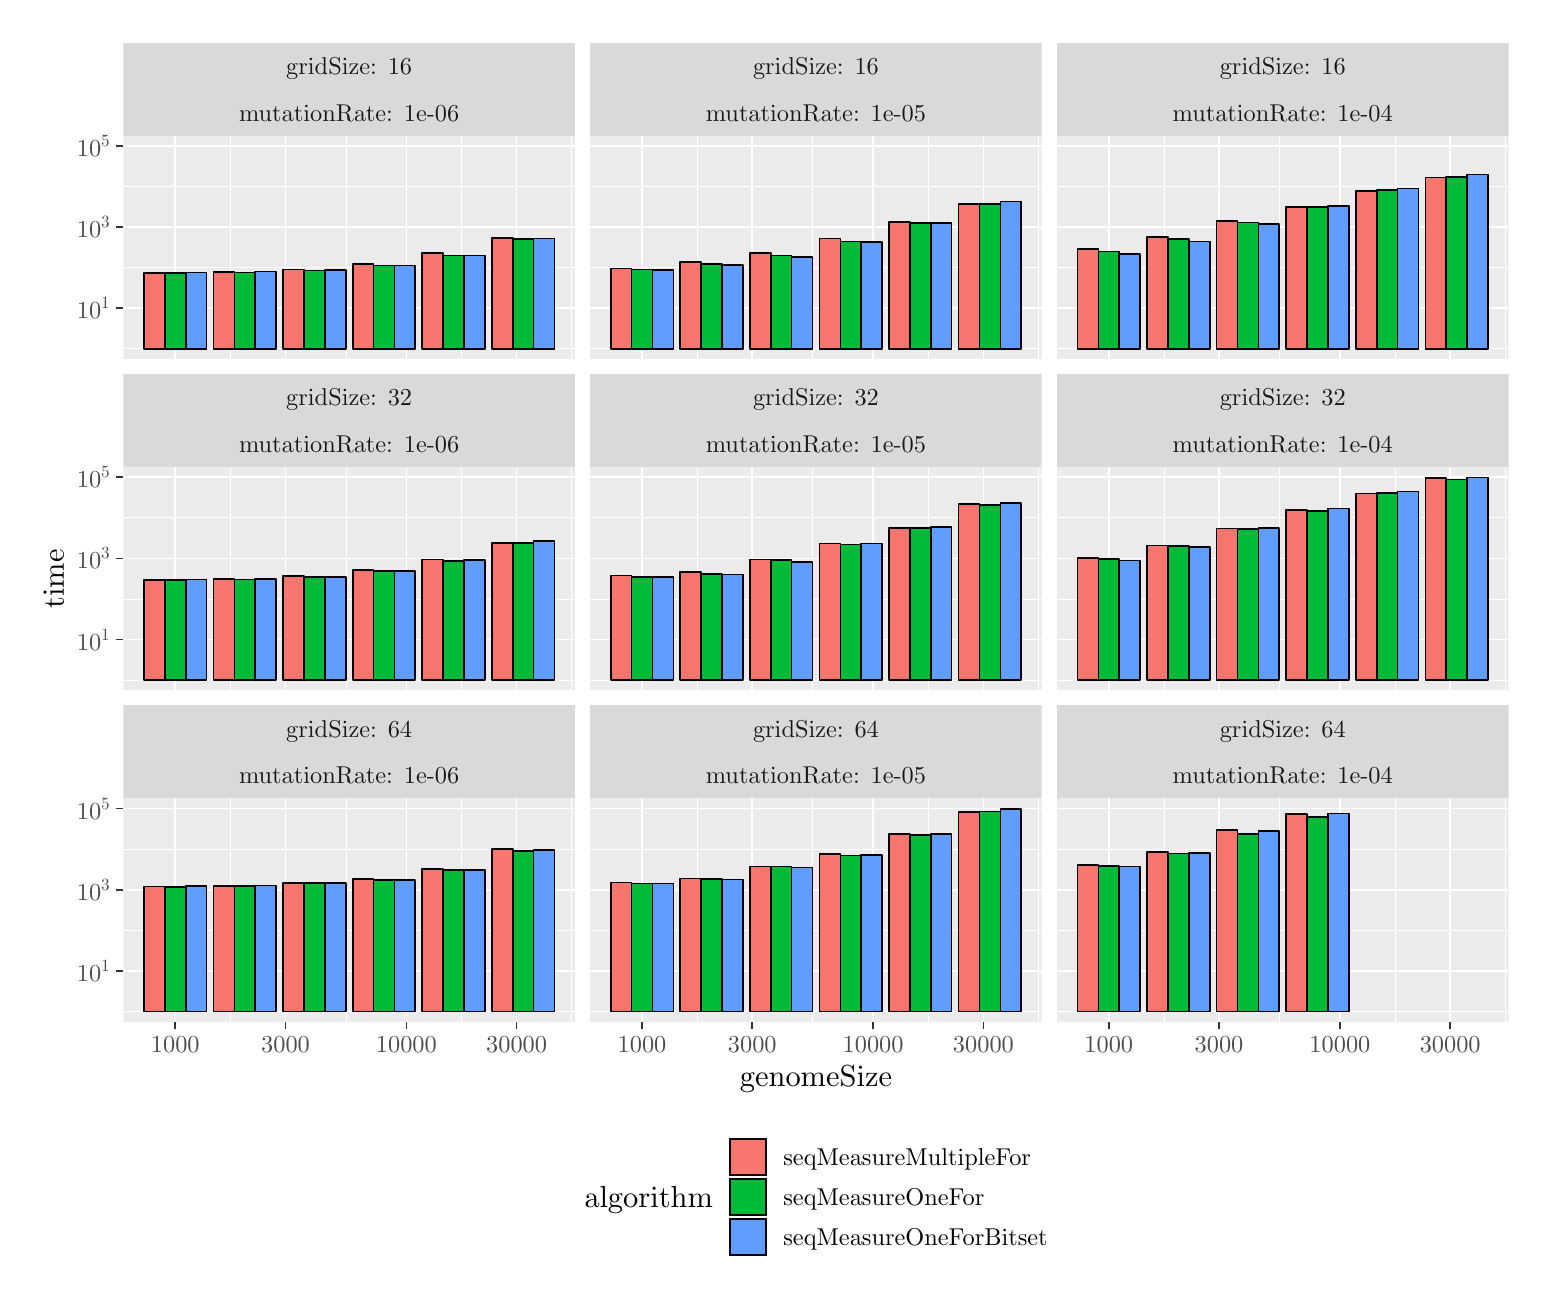
\begin{tikzpicture}[x=1pt,y=1pt]
\definecolor{fillColor}{RGB}{255,255,255}
\path[use as bounding box,fill=fillColor,fill opacity=0.00] (0,0) rectangle (540.60,455.24);
\begin{scope}
\path[clip] (  0.00,  0.00) rectangle (540.60,455.24);
\definecolor{drawColor}{RGB}{255,255,255}
\definecolor{fillColor}{RGB}{255,255,255}

\path[draw=drawColor,line width= 0.6pt,line join=round,line cap=round,fill=fillColor] (  0.00,  0.00) rectangle (540.60,455.24);
\end{scope}
\begin{scope}
\path[clip] ( 34.60,335.53) rectangle (197.77,416.13);
\definecolor{fillColor}{gray}{0.92}

\path[fill=fillColor] ( 34.60,335.53) rectangle (197.77,416.13);
\definecolor{drawColor}{RGB}{255,255,255}

\path[draw=drawColor,line width= 0.3pt,line join=round] ( 34.60,339.19) --
	(197.77,339.19);

\path[draw=drawColor,line width= 0.3pt,line join=round] ( 34.60,368.50) --
	(197.77,368.50);

\path[draw=drawColor,line width= 0.3pt,line join=round] ( 34.60,397.82) --
	(197.77,397.82);

\path[draw=drawColor,line width= 0.3pt,line join=round] ( 73.25,335.53) --
	( 73.25,416.13);

\path[draw=drawColor,line width= 0.3pt,line join=round] (115.01,335.53) --
	(115.01,416.13);

\path[draw=drawColor,line width= 0.3pt,line join=round] (156.77,335.53) --
	(156.77,416.13);

\path[draw=drawColor,line width= 0.3pt,line join=round] (196.62,335.53) --
	(196.62,416.13);

\path[draw=drawColor,line width= 0.6pt,line join=round] ( 34.60,353.85) --
	(197.77,353.85);

\path[draw=drawColor,line width= 0.6pt,line join=round] ( 34.60,383.16) --
	(197.77,383.16);

\path[draw=drawColor,line width= 0.6pt,line join=round] ( 34.60,412.48) --
	(197.77,412.48);

\path[draw=drawColor,line width= 0.6pt,line join=round] ( 53.33,335.53) --
	( 53.33,416.13);

\path[draw=drawColor,line width= 0.6pt,line join=round] ( 93.18,335.53) --
	( 93.18,416.13);

\path[draw=drawColor,line width= 0.6pt,line join=round] (136.85,335.53) --
	(136.85,416.13);

\path[draw=drawColor,line width= 0.6pt,line join=round] (176.69,335.53) --
	(176.69,416.13);
\definecolor{drawColor}{RGB}{0,0,0}
\definecolor{fillColor}{RGB}{97,156,255}

\path[draw=drawColor,line width= 0.6pt,line join=round,fill=fillColor] ( 57.10,339.19) rectangle ( 64.64,366.73);
\definecolor{fillColor}{RGB}{0,186,56}

\path[draw=drawColor,line width= 0.6pt,line join=round,fill=fillColor] ( 49.56,339.19) rectangle ( 57.10,366.57);
\definecolor{fillColor}{RGB}{248,118,109}

\path[draw=drawColor,line width= 0.6pt,line join=round,fill=fillColor] ( 42.01,339.19) rectangle ( 49.56,366.68);
\definecolor{fillColor}{RGB}{97,156,255}

\path[draw=drawColor,line width= 0.6pt,line join=round,fill=fillColor] ( 82.24,339.19) rectangle ( 89.78,367.17);
\definecolor{fillColor}{RGB}{0,186,56}

\path[draw=drawColor,line width= 0.6pt,line join=round,fill=fillColor] ( 74.70,339.19) rectangle ( 82.24,366.81);
\definecolor{fillColor}{RGB}{248,118,109}

\path[draw=drawColor,line width= 0.6pt,line join=round,fill=fillColor] ( 67.16,339.19) rectangle ( 74.70,367.04);
\definecolor{fillColor}{RGB}{97,156,255}

\path[draw=drawColor,line width= 0.6pt,line join=round,fill=fillColor] (107.38,339.19) rectangle (114.92,367.57);
\definecolor{fillColor}{RGB}{0,186,56}

\path[draw=drawColor,line width= 0.6pt,line join=round,fill=fillColor] ( 99.84,339.19) rectangle (107.38,367.48);
\definecolor{fillColor}{RGB}{248,118,109}

\path[draw=drawColor,line width= 0.6pt,line join=round,fill=fillColor] ( 92.30,339.19) rectangle ( 99.84,367.80);
\definecolor{fillColor}{RGB}{97,156,255}

\path[draw=drawColor,line width= 0.6pt,line join=round,fill=fillColor] (132.52,339.19) rectangle (140.07,369.33);
\definecolor{fillColor}{RGB}{0,186,56}

\path[draw=drawColor,line width= 0.6pt,line join=round,fill=fillColor] (124.98,339.19) rectangle (132.52,369.32);
\definecolor{fillColor}{RGB}{248,118,109}

\path[draw=drawColor,line width= 0.6pt,line join=round,fill=fillColor] (117.44,339.19) rectangle (124.98,369.93);
\definecolor{fillColor}{RGB}{97,156,255}

\path[draw=drawColor,line width= 0.6pt,line join=round,fill=fillColor] (157.66,339.19) rectangle (165.21,372.94);
\definecolor{fillColor}{RGB}{0,186,56}

\path[draw=drawColor,line width= 0.6pt,line join=round,fill=fillColor] (150.12,339.19) rectangle (157.66,372.91);
\definecolor{fillColor}{RGB}{248,118,109}

\path[draw=drawColor,line width= 0.6pt,line join=round,fill=fillColor] (142.58,339.19) rectangle (150.12,373.75);
\definecolor{fillColor}{RGB}{97,156,255}

\path[draw=drawColor,line width= 0.6pt,line join=round,fill=fillColor] (182.81,339.19) rectangle (190.35,379.08);
\definecolor{fillColor}{RGB}{0,186,56}

\path[draw=drawColor,line width= 0.6pt,line join=round,fill=fillColor] (175.26,339.19) rectangle (182.81,378.78);
\definecolor{fillColor}{RGB}{248,118,109}

\path[draw=drawColor,line width= 0.6pt,line join=round,fill=fillColor] (167.72,339.19) rectangle (175.26,379.24);
\end{scope}
\begin{scope}
\path[clip] ( 34.60,215.81) rectangle (197.77,296.42);
\definecolor{fillColor}{gray}{0.92}

\path[fill=fillColor] ( 34.60,215.81) rectangle (197.77,296.42);
\definecolor{drawColor}{RGB}{255,255,255}

\path[draw=drawColor,line width= 0.3pt,line join=round] ( 34.60,219.47) --
	(197.77,219.47);

\path[draw=drawColor,line width= 0.3pt,line join=round] ( 34.60,248.79) --
	(197.77,248.79);

\path[draw=drawColor,line width= 0.3pt,line join=round] ( 34.60,278.10) --
	(197.77,278.10);

\path[draw=drawColor,line width= 0.3pt,line join=round] ( 73.25,215.81) --
	( 73.25,296.42);

\path[draw=drawColor,line width= 0.3pt,line join=round] (115.01,215.81) --
	(115.01,296.42);

\path[draw=drawColor,line width= 0.3pt,line join=round] (156.77,215.81) --
	(156.77,296.42);

\path[draw=drawColor,line width= 0.3pt,line join=round] (196.62,215.81) --
	(196.62,296.42);

\path[draw=drawColor,line width= 0.6pt,line join=round] ( 34.60,234.13) --
	(197.77,234.13);

\path[draw=drawColor,line width= 0.6pt,line join=round] ( 34.60,263.44) --
	(197.77,263.44);

\path[draw=drawColor,line width= 0.6pt,line join=round] ( 34.60,292.76) --
	(197.77,292.76);

\path[draw=drawColor,line width= 0.6pt,line join=round] ( 53.33,215.81) --
	( 53.33,296.42);

\path[draw=drawColor,line width= 0.6pt,line join=round] ( 93.18,215.81) --
	( 93.18,296.42);

\path[draw=drawColor,line width= 0.6pt,line join=round] (136.85,215.81) --
	(136.85,296.42);

\path[draw=drawColor,line width= 0.6pt,line join=round] (176.69,215.81) --
	(176.69,296.42);
\definecolor{drawColor}{RGB}{0,0,0}
\definecolor{fillColor}{RGB}{97,156,255}

\path[draw=drawColor,line width= 0.6pt,line join=round,fill=fillColor] ( 57.10,219.47) rectangle ( 64.64,255.86);
\definecolor{fillColor}{RGB}{0,186,56}

\path[draw=drawColor,line width= 0.6pt,line join=round,fill=fillColor] ( 49.56,219.47) rectangle ( 57.10,255.65);
\definecolor{fillColor}{RGB}{248,118,109}

\path[draw=drawColor,line width= 0.6pt,line join=round,fill=fillColor] ( 42.01,219.47) rectangle ( 49.56,255.74);
\definecolor{fillColor}{RGB}{97,156,255}

\path[draw=drawColor,line width= 0.6pt,line join=round,fill=fillColor] ( 82.24,219.47) rectangle ( 89.78,256.11);
\definecolor{fillColor}{RGB}{0,186,56}

\path[draw=drawColor,line width= 0.6pt,line join=round,fill=fillColor] ( 74.70,219.47) rectangle ( 82.24,255.88);
\definecolor{fillColor}{RGB}{248,118,109}

\path[draw=drawColor,line width= 0.6pt,line join=round,fill=fillColor] ( 67.16,219.47) rectangle ( 74.70,255.99);
\definecolor{fillColor}{RGB}{97,156,255}

\path[draw=drawColor,line width= 0.6pt,line join=round,fill=fillColor] (107.38,219.47) rectangle (114.92,256.81);
\definecolor{fillColor}{RGB}{0,186,56}

\path[draw=drawColor,line width= 0.6pt,line join=round,fill=fillColor] ( 99.84,219.47) rectangle (107.38,256.72);
\definecolor{fillColor}{RGB}{248,118,109}

\path[draw=drawColor,line width= 0.6pt,line join=round,fill=fillColor] ( 92.30,219.47) rectangle ( 99.84,257.10);
\definecolor{fillColor}{RGB}{97,156,255}

\path[draw=drawColor,line width= 0.6pt,line join=round,fill=fillColor] (132.52,219.47) rectangle (140.07,258.89);
\definecolor{fillColor}{RGB}{0,186,56}

\path[draw=drawColor,line width= 0.6pt,line join=round,fill=fillColor] (124.98,219.47) rectangle (132.52,258.83);
\definecolor{fillColor}{RGB}{248,118,109}

\path[draw=drawColor,line width= 0.6pt,line join=round,fill=fillColor] (117.44,219.47) rectangle (124.98,259.22);
\definecolor{fillColor}{RGB}{97,156,255}

\path[draw=drawColor,line width= 0.6pt,line join=round,fill=fillColor] (157.66,219.47) rectangle (165.21,262.81);
\definecolor{fillColor}{RGB}{0,186,56}

\path[draw=drawColor,line width= 0.6pt,line join=round,fill=fillColor] (150.12,219.47) rectangle (157.66,262.58);
\definecolor{fillColor}{RGB}{248,118,109}

\path[draw=drawColor,line width= 0.6pt,line join=round,fill=fillColor] (142.58,219.47) rectangle (150.12,263.03);
\definecolor{fillColor}{RGB}{97,156,255}

\path[draw=drawColor,line width= 0.6pt,line join=round,fill=fillColor] (182.81,219.47) rectangle (190.35,269.65);
\definecolor{fillColor}{RGB}{0,186,56}

\path[draw=drawColor,line width= 0.6pt,line join=round,fill=fillColor] (175.26,219.47) rectangle (182.81,268.94);
\definecolor{fillColor}{RGB}{248,118,109}

\path[draw=drawColor,line width= 0.6pt,line join=round,fill=fillColor] (167.72,219.47) rectangle (175.26,269.02);
\end{scope}
\begin{scope}
\path[clip] ( 34.60, 96.09) rectangle (197.77,176.70);
\definecolor{fillColor}{gray}{0.92}

\path[fill=fillColor] ( 34.60, 96.09) rectangle (197.77,176.70);
\definecolor{drawColor}{RGB}{255,255,255}

\path[draw=drawColor,line width= 0.3pt,line join=round] ( 34.60, 99.75) --
	(197.77, 99.75);

\path[draw=drawColor,line width= 0.3pt,line join=round] ( 34.60,129.07) --
	(197.77,129.07);

\path[draw=drawColor,line width= 0.3pt,line join=round] ( 34.60,158.38) --
	(197.77,158.38);

\path[draw=drawColor,line width= 0.3pt,line join=round] ( 73.25, 96.09) --
	( 73.25,176.70);

\path[draw=drawColor,line width= 0.3pt,line join=round] (115.01, 96.09) --
	(115.01,176.70);

\path[draw=drawColor,line width= 0.3pt,line join=round] (156.77, 96.09) --
	(156.77,176.70);

\path[draw=drawColor,line width= 0.3pt,line join=round] (196.62, 96.09) --
	(196.62,176.70);

\path[draw=drawColor,line width= 0.6pt,line join=round] ( 34.60,114.41) --
	(197.77,114.41);

\path[draw=drawColor,line width= 0.6pt,line join=round] ( 34.60,143.72) --
	(197.77,143.72);

\path[draw=drawColor,line width= 0.6pt,line join=round] ( 34.60,173.04) --
	(197.77,173.04);

\path[draw=drawColor,line width= 0.6pt,line join=round] ( 53.33, 96.09) --
	( 53.33,176.70);

\path[draw=drawColor,line width= 0.6pt,line join=round] ( 93.18, 96.09) --
	( 93.18,176.70);

\path[draw=drawColor,line width= 0.6pt,line join=round] (136.85, 96.09) --
	(136.85,176.70);

\path[draw=drawColor,line width= 0.6pt,line join=round] (176.69, 96.09) --
	(176.69,176.70);
\definecolor{drawColor}{RGB}{0,0,0}
\definecolor{fillColor}{RGB}{97,156,255}

\path[draw=drawColor,line width= 0.6pt,line join=round,fill=fillColor] ( 57.10, 99.75) rectangle ( 64.64,145.10);
\definecolor{fillColor}{RGB}{0,186,56}

\path[draw=drawColor,line width= 0.6pt,line join=round,fill=fillColor] ( 49.56, 99.75) rectangle ( 57.10,144.84);
\definecolor{fillColor}{RGB}{248,118,109}

\path[draw=drawColor,line width= 0.6pt,line join=round,fill=fillColor] ( 42.01, 99.75) rectangle ( 49.56,144.89);
\definecolor{fillColor}{RGB}{97,156,255}

\path[draw=drawColor,line width= 0.6pt,line join=round,fill=fillColor] ( 82.24, 99.75) rectangle ( 89.78,145.25);
\definecolor{fillColor}{RGB}{0,186,56}

\path[draw=drawColor,line width= 0.6pt,line join=round,fill=fillColor] ( 74.70, 99.75) rectangle ( 82.24,145.11);
\definecolor{fillColor}{RGB}{248,118,109}

\path[draw=drawColor,line width= 0.6pt,line join=round,fill=fillColor] ( 67.16, 99.75) rectangle ( 74.70,145.13);
\definecolor{fillColor}{RGB}{97,156,255}

\path[draw=drawColor,line width= 0.6pt,line join=round,fill=fillColor] (107.38, 99.75) rectangle (114.92,146.08);
\definecolor{fillColor}{RGB}{0,186,56}

\path[draw=drawColor,line width= 0.6pt,line join=round,fill=fillColor] ( 99.84, 99.75) rectangle (107.38,146.10);
\definecolor{fillColor}{RGB}{248,118,109}

\path[draw=drawColor,line width= 0.6pt,line join=round,fill=fillColor] ( 92.30, 99.75) rectangle ( 99.84,146.12);
\definecolor{fillColor}{RGB}{97,156,255}

\path[draw=drawColor,line width= 0.6pt,line join=round,fill=fillColor] (132.52, 99.75) rectangle (140.07,147.34);
\definecolor{fillColor}{RGB}{0,186,56}

\path[draw=drawColor,line width= 0.6pt,line join=round,fill=fillColor] (124.98, 99.75) rectangle (132.52,147.36);
\definecolor{fillColor}{RGB}{248,118,109}

\path[draw=drawColor,line width= 0.6pt,line join=round,fill=fillColor] (117.44, 99.75) rectangle (124.98,147.56);
\definecolor{fillColor}{RGB}{97,156,255}

\path[draw=drawColor,line width= 0.6pt,line join=round,fill=fillColor] (157.66, 99.75) rectangle (165.21,150.95);
\definecolor{fillColor}{RGB}{0,186,56}

\path[draw=drawColor,line width= 0.6pt,line join=round,fill=fillColor] (150.12, 99.75) rectangle (157.66,150.79);
\definecolor{fillColor}{RGB}{248,118,109}

\path[draw=drawColor,line width= 0.6pt,line join=round,fill=fillColor] (142.58, 99.75) rectangle (150.12,151.21);
\definecolor{fillColor}{RGB}{97,156,255}

\path[draw=drawColor,line width= 0.6pt,line join=round,fill=fillColor] (182.81, 99.75) rectangle (190.35,158.15);
\definecolor{fillColor}{RGB}{0,186,56}

\path[draw=drawColor,line width= 0.6pt,line join=round,fill=fillColor] (175.26, 99.75) rectangle (182.81,157.63);
\definecolor{fillColor}{RGB}{248,118,109}

\path[draw=drawColor,line width= 0.6pt,line join=round,fill=fillColor] (167.72, 99.75) rectangle (175.26,158.41);
\end{scope}
\begin{scope}
\path[clip] (203.27,335.53) rectangle (366.43,416.13);
\definecolor{fillColor}{gray}{0.92}

\path[fill=fillColor] (203.27,335.53) rectangle (366.43,416.13);
\definecolor{drawColor}{RGB}{255,255,255}

\path[draw=drawColor,line width= 0.3pt,line join=round] (203.27,339.19) --
	(366.43,339.19);

\path[draw=drawColor,line width= 0.3pt,line join=round] (203.27,368.50) --
	(366.43,368.50);

\path[draw=drawColor,line width= 0.3pt,line join=round] (203.27,397.82) --
	(366.43,397.82);

\path[draw=drawColor,line width= 0.3pt,line join=round] (241.92,335.53) --
	(241.92,416.13);

\path[draw=drawColor,line width= 0.3pt,line join=round] (283.68,335.53) --
	(283.68,416.13);

\path[draw=drawColor,line width= 0.3pt,line join=round] (325.44,335.53) --
	(325.44,416.13);

\path[draw=drawColor,line width= 0.3pt,line join=round] (365.29,335.53) --
	(365.29,416.13);

\path[draw=drawColor,line width= 0.6pt,line join=round] (203.27,353.85) --
	(366.43,353.85);

\path[draw=drawColor,line width= 0.6pt,line join=round] (203.27,383.16) --
	(366.43,383.16);

\path[draw=drawColor,line width= 0.6pt,line join=round] (203.27,412.48) --
	(366.43,412.48);

\path[draw=drawColor,line width= 0.6pt,line join=round] (222.00,335.53) --
	(222.00,416.13);

\path[draw=drawColor,line width= 0.6pt,line join=round] (261.84,335.53) --
	(261.84,416.13);

\path[draw=drawColor,line width= 0.6pt,line join=round] (305.51,335.53) --
	(305.51,416.13);

\path[draw=drawColor,line width= 0.6pt,line join=round] (345.36,335.53) --
	(345.36,416.13);
\definecolor{drawColor}{RGB}{0,0,0}
\definecolor{fillColor}{RGB}{97,156,255}

\path[draw=drawColor,line width= 0.6pt,line join=round,fill=fillColor] (225.77,339.19) rectangle (233.31,367.70);
\definecolor{fillColor}{RGB}{0,186,56}

\path[draw=drawColor,line width= 0.6pt,line join=round,fill=fillColor] (218.22,339.19) rectangle (225.77,367.84);
\definecolor{fillColor}{RGB}{248,118,109}

\path[draw=drawColor,line width= 0.6pt,line join=round,fill=fillColor] (210.68,339.19) rectangle (218.22,368.26);
\definecolor{fillColor}{RGB}{97,156,255}

\path[draw=drawColor,line width= 0.6pt,line join=round,fill=fillColor] (250.91,339.19) rectangle (258.45,369.57);
\definecolor{fillColor}{RGB}{0,186,56}

\path[draw=drawColor,line width= 0.6pt,line join=round,fill=fillColor] (243.37,339.19) rectangle (250.91,369.95);
\definecolor{fillColor}{RGB}{248,118,109}

\path[draw=drawColor,line width= 0.6pt,line join=round,fill=fillColor] (235.82,339.19) rectangle (243.37,370.62);
\definecolor{fillColor}{RGB}{97,156,255}

\path[draw=drawColor,line width= 0.6pt,line join=round,fill=fillColor] (276.05,339.19) rectangle (283.59,372.45);
\definecolor{fillColor}{RGB}{0,186,56}

\path[draw=drawColor,line width= 0.6pt,line join=round,fill=fillColor] (268.51,339.19) rectangle (276.05,372.92);
\definecolor{fillColor}{RGB}{248,118,109}

\path[draw=drawColor,line width= 0.6pt,line join=round,fill=fillColor] (260.97,339.19) rectangle (268.51,373.89);
\definecolor{fillColor}{RGB}{97,156,255}

\path[draw=drawColor,line width= 0.6pt,line join=round,fill=fillColor] (301.19,339.19) rectangle (308.73,377.67);
\definecolor{fillColor}{RGB}{0,186,56}

\path[draw=drawColor,line width= 0.6pt,line join=round,fill=fillColor] (293.65,339.19) rectangle (301.19,377.92);
\definecolor{fillColor}{RGB}{248,118,109}

\path[draw=drawColor,line width= 0.6pt,line join=round,fill=fillColor] (286.11,339.19) rectangle (293.65,379.05);
\definecolor{fillColor}{RGB}{97,156,255}

\path[draw=drawColor,line width= 0.6pt,line join=round,fill=fillColor] (326.33,339.19) rectangle (333.88,384.75);
\definecolor{fillColor}{RGB}{0,186,56}

\path[draw=drawColor,line width= 0.6pt,line join=round,fill=fillColor] (318.79,339.19) rectangle (326.33,384.57);
\definecolor{fillColor}{RGB}{248,118,109}

\path[draw=drawColor,line width= 0.6pt,line join=round,fill=fillColor] (311.25,339.19) rectangle (318.79,385.02);
\definecolor{fillColor}{RGB}{97,156,255}

\path[draw=drawColor,line width= 0.6pt,line join=round,fill=fillColor] (351.47,339.19) rectangle (359.02,392.48);
\definecolor{fillColor}{RGB}{0,186,56}

\path[draw=drawColor,line width= 0.6pt,line join=round,fill=fillColor] (343.93,339.19) rectangle (351.47,391.52);
\definecolor{fillColor}{RGB}{248,118,109}

\path[draw=drawColor,line width= 0.6pt,line join=round,fill=fillColor] (336.39,339.19) rectangle (343.93,391.50);
\end{scope}
\begin{scope}
\path[clip] (203.27,215.81) rectangle (366.43,296.42);
\definecolor{fillColor}{gray}{0.92}

\path[fill=fillColor] (203.27,215.81) rectangle (366.43,296.42);
\definecolor{drawColor}{RGB}{255,255,255}

\path[draw=drawColor,line width= 0.3pt,line join=round] (203.27,219.47) --
	(366.43,219.47);

\path[draw=drawColor,line width= 0.3pt,line join=round] (203.27,248.79) --
	(366.43,248.79);

\path[draw=drawColor,line width= 0.3pt,line join=round] (203.27,278.10) --
	(366.43,278.10);

\path[draw=drawColor,line width= 0.3pt,line join=round] (241.92,215.81) --
	(241.92,296.42);

\path[draw=drawColor,line width= 0.3pt,line join=round] (283.68,215.81) --
	(283.68,296.42);

\path[draw=drawColor,line width= 0.3pt,line join=round] (325.44,215.81) --
	(325.44,296.42);

\path[draw=drawColor,line width= 0.3pt,line join=round] (365.29,215.81) --
	(365.29,296.42);

\path[draw=drawColor,line width= 0.6pt,line join=round] (203.27,234.13) --
	(366.43,234.13);

\path[draw=drawColor,line width= 0.6pt,line join=round] (203.27,263.44) --
	(366.43,263.44);

\path[draw=drawColor,line width= 0.6pt,line join=round] (203.27,292.76) --
	(366.43,292.76);

\path[draw=drawColor,line width= 0.6pt,line join=round] (222.00,215.81) --
	(222.00,296.42);

\path[draw=drawColor,line width= 0.6pt,line join=round] (261.84,215.81) --
	(261.84,296.42);

\path[draw=drawColor,line width= 0.6pt,line join=round] (305.51,215.81) --
	(305.51,296.42);

\path[draw=drawColor,line width= 0.6pt,line join=round] (345.36,215.81) --
	(345.36,296.42);
\definecolor{drawColor}{RGB}{0,0,0}
\definecolor{fillColor}{RGB}{97,156,255}

\path[draw=drawColor,line width= 0.6pt,line join=round,fill=fillColor] (225.77,219.47) rectangle (233.31,256.75);
\definecolor{fillColor}{RGB}{0,186,56}

\path[draw=drawColor,line width= 0.6pt,line join=round,fill=fillColor] (218.22,219.47) rectangle (225.77,256.80);
\definecolor{fillColor}{RGB}{248,118,109}

\path[draw=drawColor,line width= 0.6pt,line join=round,fill=fillColor] (210.68,219.47) rectangle (218.22,257.22);
\definecolor{fillColor}{RGB}{97,156,255}

\path[draw=drawColor,line width= 0.6pt,line join=round,fill=fillColor] (250.91,219.47) rectangle (258.45,257.68);
\definecolor{fillColor}{RGB}{0,186,56}

\path[draw=drawColor,line width= 0.6pt,line join=round,fill=fillColor] (243.37,219.47) rectangle (250.91,257.90);
\definecolor{fillColor}{RGB}{248,118,109}

\path[draw=drawColor,line width= 0.6pt,line join=round,fill=fillColor] (235.82,219.47) rectangle (243.37,258.58);
\definecolor{fillColor}{RGB}{97,156,255}

\path[draw=drawColor,line width= 0.6pt,line join=round,fill=fillColor] (276.05,219.47) rectangle (283.59,262.10);
\definecolor{fillColor}{RGB}{0,186,56}

\path[draw=drawColor,line width= 0.6pt,line join=round,fill=fillColor] (268.51,219.47) rectangle (276.05,262.81);
\definecolor{fillColor}{RGB}{248,118,109}

\path[draw=drawColor,line width= 0.6pt,line join=round,fill=fillColor] (260.97,219.47) rectangle (268.51,263.04);
\definecolor{fillColor}{RGB}{97,156,255}

\path[draw=drawColor,line width= 0.6pt,line join=round,fill=fillColor] (301.19,219.47) rectangle (308.73,268.89);
\definecolor{fillColor}{RGB}{0,186,56}

\path[draw=drawColor,line width= 0.6pt,line join=round,fill=fillColor] (293.65,219.47) rectangle (301.19,268.48);
\definecolor{fillColor}{RGB}{248,118,109}

\path[draw=drawColor,line width= 0.6pt,line join=round,fill=fillColor] (286.11,219.47) rectangle (293.65,268.81);
\definecolor{fillColor}{RGB}{97,156,255}

\path[draw=drawColor,line width= 0.6pt,line join=round,fill=fillColor] (326.33,219.47) rectangle (333.88,274.88);
\definecolor{fillColor}{RGB}{0,186,56}

\path[draw=drawColor,line width= 0.6pt,line join=round,fill=fillColor] (318.79,219.47) rectangle (326.33,274.38);
\definecolor{fillColor}{RGB}{248,118,109}

\path[draw=drawColor,line width= 0.6pt,line join=round,fill=fillColor] (311.25,219.47) rectangle (318.79,274.53);
\definecolor{fillColor}{RGB}{97,156,255}

\path[draw=drawColor,line width= 0.6pt,line join=round,fill=fillColor] (351.47,219.47) rectangle (359.02,283.59);
\definecolor{fillColor}{RGB}{0,186,56}

\path[draw=drawColor,line width= 0.6pt,line join=round,fill=fillColor] (343.93,219.47) rectangle (351.47,282.86);
\definecolor{fillColor}{RGB}{248,118,109}

\path[draw=drawColor,line width= 0.6pt,line join=round,fill=fillColor] (336.39,219.47) rectangle (343.93,283.19);
\end{scope}
\begin{scope}
\path[clip] (203.27, 96.09) rectangle (366.43,176.70);
\definecolor{fillColor}{gray}{0.92}

\path[fill=fillColor] (203.27, 96.09) rectangle (366.43,176.70);
\definecolor{drawColor}{RGB}{255,255,255}

\path[draw=drawColor,line width= 0.3pt,line join=round] (203.27, 99.75) --
	(366.43, 99.75);

\path[draw=drawColor,line width= 0.3pt,line join=round] (203.27,129.07) --
	(366.43,129.07);

\path[draw=drawColor,line width= 0.3pt,line join=round] (203.27,158.38) --
	(366.43,158.38);

\path[draw=drawColor,line width= 0.3pt,line join=round] (241.92, 96.09) --
	(241.92,176.70);

\path[draw=drawColor,line width= 0.3pt,line join=round] (283.68, 96.09) --
	(283.68,176.70);

\path[draw=drawColor,line width= 0.3pt,line join=round] (325.44, 96.09) --
	(325.44,176.70);

\path[draw=drawColor,line width= 0.3pt,line join=round] (365.29, 96.09) --
	(365.29,176.70);

\path[draw=drawColor,line width= 0.6pt,line join=round] (203.27,114.41) --
	(366.43,114.41);

\path[draw=drawColor,line width= 0.6pt,line join=round] (203.27,143.72) --
	(366.43,143.72);

\path[draw=drawColor,line width= 0.6pt,line join=round] (203.27,173.04) --
	(366.43,173.04);

\path[draw=drawColor,line width= 0.6pt,line join=round] (222.00, 96.09) --
	(222.00,176.70);

\path[draw=drawColor,line width= 0.6pt,line join=round] (261.84, 96.09) --
	(261.84,176.70);

\path[draw=drawColor,line width= 0.6pt,line join=round] (305.51, 96.09) --
	(305.51,176.70);

\path[draw=drawColor,line width= 0.6pt,line join=round] (345.36, 96.09) --
	(345.36,176.70);
\definecolor{drawColor}{RGB}{0,0,0}
\definecolor{fillColor}{RGB}{97,156,255}

\path[draw=drawColor,line width= 0.6pt,line join=round,fill=fillColor] (225.77, 99.75) rectangle (233.31,146.00);
\definecolor{fillColor}{RGB}{0,186,56}

\path[draw=drawColor,line width= 0.6pt,line join=round,fill=fillColor] (218.22, 99.75) rectangle (225.77,146.04);
\definecolor{fillColor}{RGB}{248,118,109}

\path[draw=drawColor,line width= 0.6pt,line join=round,fill=fillColor] (210.68, 99.75) rectangle (218.22,146.29);
\definecolor{fillColor}{RGB}{97,156,255}

\path[draw=drawColor,line width= 0.6pt,line join=round,fill=fillColor] (250.91, 99.75) rectangle (258.45,147.49);
\definecolor{fillColor}{RGB}{0,186,56}

\path[draw=drawColor,line width= 0.6pt,line join=round,fill=fillColor] (243.37, 99.75) rectangle (250.91,147.68);
\definecolor{fillColor}{RGB}{248,118,109}

\path[draw=drawColor,line width= 0.6pt,line join=round,fill=fillColor] (235.82, 99.75) rectangle (243.37,147.80);
\definecolor{fillColor}{RGB}{97,156,255}

\path[draw=drawColor,line width= 0.6pt,line join=round,fill=fillColor] (276.05, 99.75) rectangle (283.59,151.82);
\definecolor{fillColor}{RGB}{0,186,56}

\path[draw=drawColor,line width= 0.6pt,line join=round,fill=fillColor] (268.51, 99.75) rectangle (276.05,152.17);
\definecolor{fillColor}{RGB}{248,118,109}

\path[draw=drawColor,line width= 0.6pt,line join=round,fill=fillColor] (260.97, 99.75) rectangle (268.51,152.17);
\definecolor{fillColor}{RGB}{97,156,255}

\path[draw=drawColor,line width= 0.6pt,line join=round,fill=fillColor] (301.19, 99.75) rectangle (308.73,156.40);
\definecolor{fillColor}{RGB}{0,186,56}

\path[draw=drawColor,line width= 0.6pt,line join=round,fill=fillColor] (293.65, 99.75) rectangle (301.19,156.10);
\definecolor{fillColor}{RGB}{248,118,109}

\path[draw=drawColor,line width= 0.6pt,line join=round,fill=fillColor] (286.11, 99.75) rectangle (293.65,156.74);
\definecolor{fillColor}{RGB}{97,156,255}

\path[draw=drawColor,line width= 0.6pt,line join=round,fill=fillColor] (326.33, 99.75) rectangle (333.88,163.89);
\definecolor{fillColor}{RGB}{0,186,56}

\path[draw=drawColor,line width= 0.6pt,line join=round,fill=fillColor] (318.79, 99.75) rectangle (326.33,163.41);
\definecolor{fillColor}{RGB}{248,118,109}

\path[draw=drawColor,line width= 0.6pt,line join=round,fill=fillColor] (311.25, 99.75) rectangle (318.79,163.87);
\definecolor{fillColor}{RGB}{97,156,255}

\path[draw=drawColor,line width= 0.6pt,line join=round,fill=fillColor] (351.47, 99.75) rectangle (359.02,172.93);
\definecolor{fillColor}{RGB}{0,186,56}

\path[draw=drawColor,line width= 0.6pt,line join=round,fill=fillColor] (343.93, 99.75) rectangle (351.47,172.04);
\definecolor{fillColor}{RGB}{248,118,109}

\path[draw=drawColor,line width= 0.6pt,line join=round,fill=fillColor] (336.39, 99.75) rectangle (343.93,171.87);
\end{scope}
\begin{scope}
\path[clip] (371.93,335.53) rectangle (535.10,416.13);
\definecolor{fillColor}{gray}{0.92}

\path[fill=fillColor] (371.93,335.53) rectangle (535.10,416.13);
\definecolor{drawColor}{RGB}{255,255,255}

\path[draw=drawColor,line width= 0.3pt,line join=round] (371.93,339.19) --
	(535.10,339.19);

\path[draw=drawColor,line width= 0.3pt,line join=round] (371.93,368.50) --
	(535.10,368.50);

\path[draw=drawColor,line width= 0.3pt,line join=round] (371.93,397.82) --
	(535.10,397.82);

\path[draw=drawColor,line width= 0.3pt,line join=round] (410.59,335.53) --
	(410.59,416.13);

\path[draw=drawColor,line width= 0.3pt,line join=round] (452.35,335.53) --
	(452.35,416.13);

\path[draw=drawColor,line width= 0.3pt,line join=round] (494.11,335.53) --
	(494.11,416.13);

\path[draw=drawColor,line width= 0.3pt,line join=round] (533.96,335.53) --
	(533.96,416.13);

\path[draw=drawColor,line width= 0.6pt,line join=round] (371.93,353.85) --
	(535.10,353.85);

\path[draw=drawColor,line width= 0.6pt,line join=round] (371.93,383.16) --
	(535.10,383.16);

\path[draw=drawColor,line width= 0.6pt,line join=round] (371.93,412.48) --
	(535.10,412.48);

\path[draw=drawColor,line width= 0.6pt,line join=round] (390.66,335.53) --
	(390.66,416.13);

\path[draw=drawColor,line width= 0.6pt,line join=round] (430.51,335.53) --
	(430.51,416.13);

\path[draw=drawColor,line width= 0.6pt,line join=round] (474.18,335.53) --
	(474.18,416.13);

\path[draw=drawColor,line width= 0.6pt,line join=round] (514.03,335.53) --
	(514.03,416.13);
\definecolor{drawColor}{RGB}{0,0,0}
\definecolor{fillColor}{RGB}{97,156,255}

\path[draw=drawColor,line width= 0.6pt,line join=round,fill=fillColor] (394.44,339.19) rectangle (401.98,373.40);
\definecolor{fillColor}{RGB}{0,186,56}

\path[draw=drawColor,line width= 0.6pt,line join=round,fill=fillColor] (386.89,339.19) rectangle (394.44,374.36);
\definecolor{fillColor}{RGB}{248,118,109}

\path[draw=drawColor,line width= 0.6pt,line join=round,fill=fillColor] (379.35,339.19) rectangle (386.89,375.18);
\definecolor{fillColor}{RGB}{97,156,255}

\path[draw=drawColor,line width= 0.6pt,line join=round,fill=fillColor] (419.58,339.19) rectangle (427.12,377.92);
\definecolor{fillColor}{RGB}{0,186,56}

\path[draw=drawColor,line width= 0.6pt,line join=round,fill=fillColor] (412.03,339.19) rectangle (419.58,378.85);
\definecolor{fillColor}{RGB}{248,118,109}

\path[draw=drawColor,line width= 0.6pt,line join=round,fill=fillColor] (404.49,339.19) rectangle (412.03,379.66);
\definecolor{fillColor}{RGB}{97,156,255}

\path[draw=drawColor,line width= 0.6pt,line join=round,fill=fillColor] (444.72,339.19) rectangle (452.26,384.21);
\definecolor{fillColor}{RGB}{0,186,56}

\path[draw=drawColor,line width= 0.6pt,line join=round,fill=fillColor] (437.18,339.19) rectangle (444.72,384.89);
\definecolor{fillColor}{RGB}{248,118,109}

\path[draw=drawColor,line width= 0.6pt,line join=round,fill=fillColor] (429.63,339.19) rectangle (437.18,385.32);
\definecolor{fillColor}{RGB}{97,156,255}

\path[draw=drawColor,line width= 0.6pt,line join=round,fill=fillColor] (469.86,339.19) rectangle (477.40,390.78);
\definecolor{fillColor}{RGB}{0,186,56}

\path[draw=drawColor,line width= 0.6pt,line join=round,fill=fillColor] (462.32,339.19) rectangle (469.86,390.55);
\definecolor{fillColor}{RGB}{248,118,109}

\path[draw=drawColor,line width= 0.6pt,line join=round,fill=fillColor] (454.78,339.19) rectangle (462.32,390.49);
\definecolor{fillColor}{RGB}{97,156,255}

\path[draw=drawColor,line width= 0.6pt,line join=round,fill=fillColor] (495.00,339.19) rectangle (502.54,397.09);
\definecolor{fillColor}{RGB}{0,186,56}

\path[draw=drawColor,line width= 0.6pt,line join=round,fill=fillColor] (487.46,339.19) rectangle (495.00,396.46);
\definecolor{fillColor}{RGB}{248,118,109}

\path[draw=drawColor,line width= 0.6pt,line join=round,fill=fillColor] (479.92,339.19) rectangle (487.46,396.31);
\definecolor{fillColor}{RGB}{97,156,255}

\path[draw=drawColor,line width= 0.6pt,line join=round,fill=fillColor] (520.14,339.19) rectangle (527.69,402.13);
\definecolor{fillColor}{RGB}{0,186,56}

\path[draw=drawColor,line width= 0.6pt,line join=round,fill=fillColor] (512.60,339.19) rectangle (520.14,401.27);
\definecolor{fillColor}{RGB}{248,118,109}

\path[draw=drawColor,line width= 0.6pt,line join=round,fill=fillColor] (505.06,339.19) rectangle (512.60,401.15);
\end{scope}
\begin{scope}
\path[clip] (371.93,215.81) rectangle (535.10,296.42);
\definecolor{fillColor}{gray}{0.92}

\path[fill=fillColor] (371.93,215.81) rectangle (535.10,296.42);
\definecolor{drawColor}{RGB}{255,255,255}

\path[draw=drawColor,line width= 0.3pt,line join=round] (371.93,219.47) --
	(535.10,219.47);

\path[draw=drawColor,line width= 0.3pt,line join=round] (371.93,248.79) --
	(535.10,248.79);

\path[draw=drawColor,line width= 0.3pt,line join=round] (371.93,278.10) --
	(535.10,278.10);

\path[draw=drawColor,line width= 0.3pt,line join=round] (410.59,215.81) --
	(410.59,296.42);

\path[draw=drawColor,line width= 0.3pt,line join=round] (452.35,215.81) --
	(452.35,296.42);

\path[draw=drawColor,line width= 0.3pt,line join=round] (494.11,215.81) --
	(494.11,296.42);

\path[draw=drawColor,line width= 0.3pt,line join=round] (533.96,215.81) --
	(533.96,296.42);

\path[draw=drawColor,line width= 0.6pt,line join=round] (371.93,234.13) --
	(535.10,234.13);

\path[draw=drawColor,line width= 0.6pt,line join=round] (371.93,263.44) --
	(535.10,263.44);

\path[draw=drawColor,line width= 0.6pt,line join=round] (371.93,292.76) --
	(535.10,292.76);

\path[draw=drawColor,line width= 0.6pt,line join=round] (390.66,215.81) --
	(390.66,296.42);

\path[draw=drawColor,line width= 0.6pt,line join=round] (430.51,215.81) --
	(430.51,296.42);

\path[draw=drawColor,line width= 0.6pt,line join=round] (474.18,215.81) --
	(474.18,296.42);

\path[draw=drawColor,line width= 0.6pt,line join=round] (514.03,215.81) --
	(514.03,296.42);
\definecolor{drawColor}{RGB}{0,0,0}
\definecolor{fillColor}{RGB}{97,156,255}

\path[draw=drawColor,line width= 0.6pt,line join=round,fill=fillColor] (394.44,219.47) rectangle (401.98,262.75);
\definecolor{fillColor}{RGB}{0,186,56}

\path[draw=drawColor,line width= 0.6pt,line join=round,fill=fillColor] (386.89,219.47) rectangle (394.44,263.30);
\definecolor{fillColor}{RGB}{248,118,109}

\path[draw=drawColor,line width= 0.6pt,line join=round,fill=fillColor] (379.35,219.47) rectangle (386.89,263.72);
\definecolor{fillColor}{RGB}{97,156,255}

\path[draw=drawColor,line width= 0.6pt,line join=round,fill=fillColor] (419.58,219.47) rectangle (427.12,267.63);
\definecolor{fillColor}{RGB}{0,186,56}

\path[draw=drawColor,line width= 0.6pt,line join=round,fill=fillColor] (412.03,219.47) rectangle (419.58,267.96);
\definecolor{fillColor}{RGB}{248,118,109}

\path[draw=drawColor,line width= 0.6pt,line join=round,fill=fillColor] (404.49,219.47) rectangle (412.03,268.10);
\definecolor{fillColor}{RGB}{97,156,255}

\path[draw=drawColor,line width= 0.6pt,line join=round,fill=fillColor] (444.72,219.47) rectangle (452.26,274.45);
\definecolor{fillColor}{RGB}{0,186,56}

\path[draw=drawColor,line width= 0.6pt,line join=round,fill=fillColor] (437.18,219.47) rectangle (444.72,274.16);
\definecolor{fillColor}{RGB}{248,118,109}

\path[draw=drawColor,line width= 0.6pt,line join=round,fill=fillColor] (429.63,219.47) rectangle (437.18,274.24);
\definecolor{fillColor}{RGB}{97,156,255}

\path[draw=drawColor,line width= 0.6pt,line join=round,fill=fillColor] (469.86,219.47) rectangle (477.40,281.48);
\definecolor{fillColor}{RGB}{0,186,56}

\path[draw=drawColor,line width= 0.6pt,line join=round,fill=fillColor] (462.32,219.47) rectangle (469.86,280.48);
\definecolor{fillColor}{RGB}{248,118,109}

\path[draw=drawColor,line width= 0.6pt,line join=round,fill=fillColor] (454.78,219.47) rectangle (462.32,280.89);
\definecolor{fillColor}{RGB}{97,156,255}

\path[draw=drawColor,line width= 0.6pt,line join=round,fill=fillColor] (495.00,219.47) rectangle (502.54,287.65);
\definecolor{fillColor}{RGB}{0,186,56}

\path[draw=drawColor,line width= 0.6pt,line join=round,fill=fillColor] (487.46,219.47) rectangle (495.00,287.18);
\definecolor{fillColor}{RGB}{248,118,109}

\path[draw=drawColor,line width= 0.6pt,line join=round,fill=fillColor] (479.92,219.47) rectangle (487.46,286.93);
\definecolor{fillColor}{RGB}{97,156,255}

\path[draw=drawColor,line width= 0.6pt,line join=round,fill=fillColor] (520.14,219.47) rectangle (527.69,292.75);
\definecolor{fillColor}{RGB}{0,186,56}

\path[draw=drawColor,line width= 0.6pt,line join=round,fill=fillColor] (512.60,219.47) rectangle (520.14,291.92);
\definecolor{fillColor}{RGB}{248,118,109}

\path[draw=drawColor,line width= 0.6pt,line join=round,fill=fillColor] (505.06,219.47) rectangle (512.60,292.49);
\end{scope}
\begin{scope}
\path[clip] (371.93, 96.09) rectangle (535.10,176.70);
\definecolor{fillColor}{gray}{0.92}

\path[fill=fillColor] (371.93, 96.09) rectangle (535.10,176.70);
\definecolor{drawColor}{RGB}{255,255,255}

\path[draw=drawColor,line width= 0.3pt,line join=round] (371.93, 99.75) --
	(535.10, 99.75);

\path[draw=drawColor,line width= 0.3pt,line join=round] (371.93,129.07) --
	(535.10,129.07);

\path[draw=drawColor,line width= 0.3pt,line join=round] (371.93,158.38) --
	(535.10,158.38);

\path[draw=drawColor,line width= 0.3pt,line join=round] (410.59, 96.09) --
	(410.59,176.70);

\path[draw=drawColor,line width= 0.3pt,line join=round] (452.35, 96.09) --
	(452.35,176.70);

\path[draw=drawColor,line width= 0.3pt,line join=round] (494.11, 96.09) --
	(494.11,176.70);

\path[draw=drawColor,line width= 0.3pt,line join=round] (533.96, 96.09) --
	(533.96,176.70);

\path[draw=drawColor,line width= 0.6pt,line join=round] (371.93,114.41) --
	(535.10,114.41);

\path[draw=drawColor,line width= 0.6pt,line join=round] (371.93,143.72) --
	(535.10,143.72);

\path[draw=drawColor,line width= 0.6pt,line join=round] (371.93,173.04) --
	(535.10,173.04);

\path[draw=drawColor,line width= 0.6pt,line join=round] (390.66, 96.09) --
	(390.66,176.70);

\path[draw=drawColor,line width= 0.6pt,line join=round] (430.51, 96.09) --
	(430.51,176.70);

\path[draw=drawColor,line width= 0.6pt,line join=round] (474.18, 96.09) --
	(474.18,176.70);

\path[draw=drawColor,line width= 0.6pt,line join=round] (514.03, 96.09) --
	(514.03,176.70);
\definecolor{drawColor}{RGB}{0,0,0}
\definecolor{fillColor}{RGB}{97,156,255}

\path[draw=drawColor,line width= 0.6pt,line join=round,fill=fillColor] (394.44, 99.75) rectangle (401.98,152.11);
\definecolor{fillColor}{RGB}{0,186,56}

\path[draw=drawColor,line width= 0.6pt,line join=round,fill=fillColor] (386.89, 99.75) rectangle (394.44,152.41);
\definecolor{fillColor}{RGB}{248,118,109}

\path[draw=drawColor,line width= 0.6pt,line join=round,fill=fillColor] (379.35, 99.75) rectangle (386.89,152.62);
\definecolor{fillColor}{RGB}{97,156,255}

\path[draw=drawColor,line width= 0.6pt,line join=round,fill=fillColor] (419.58, 99.75) rectangle (427.12,156.99);
\definecolor{fillColor}{RGB}{0,186,56}

\path[draw=drawColor,line width= 0.6pt,line join=round,fill=fillColor] (412.03, 99.75) rectangle (419.58,156.84);
\definecolor{fillColor}{RGB}{248,118,109}

\path[draw=drawColor,line width= 0.6pt,line join=round,fill=fillColor] (404.49, 99.75) rectangle (412.03,157.35);
\definecolor{fillColor}{RGB}{97,156,255}

\path[draw=drawColor,line width= 0.6pt,line join=round,fill=fillColor] (444.72, 99.75) rectangle (452.26,165.07);
\definecolor{fillColor}{RGB}{0,186,56}

\path[draw=drawColor,line width= 0.6pt,line join=round,fill=fillColor] (437.18, 99.75) rectangle (444.72,163.87);
\definecolor{fillColor}{RGB}{248,118,109}

\path[draw=drawColor,line width= 0.6pt,line join=round,fill=fillColor] (429.63, 99.75) rectangle (437.18,165.22);
\definecolor{fillColor}{RGB}{97,156,255}

\path[draw=drawColor,line width= 0.6pt,line join=round,fill=fillColor] (469.86, 99.75) rectangle (477.40,171.23);
\definecolor{fillColor}{RGB}{0,186,56}

\path[draw=drawColor,line width= 0.6pt,line join=round,fill=fillColor] (462.32, 99.75) rectangle (469.86,169.93);
\definecolor{fillColor}{RGB}{248,118,109}

\path[draw=drawColor,line width= 0.6pt,line join=round,fill=fillColor] (454.78, 99.75) rectangle (462.32,171.05);
\end{scope}
\begin{scope}
\path[clip] ( 34.60,193.50) rectangle (197.77,210.31);
\definecolor{fillColor}{gray}{0.85}

\path[fill=fillColor] ( 34.60,193.50) rectangle (197.77,210.31);
\definecolor{drawColor}{gray}{0.10}

\node[text=drawColor,anchor=base,inner sep=0pt, outer sep=0pt, scale=  0.88] at (116.18,198.87) {gridSize: 64};
\end{scope}
\begin{scope}
\path[clip] ( 34.60,176.70) rectangle (197.77,193.50);
\definecolor{fillColor}{gray}{0.85}

\path[fill=fillColor] ( 34.60,176.70) rectangle (197.77,193.50);
\definecolor{drawColor}{gray}{0.10}

\node[text=drawColor,anchor=base,inner sep=0pt, outer sep=0pt, scale=  0.88] at (116.18,182.07) {mutationRate: 1e-06};
\end{scope}
\begin{scope}
\path[clip] (203.27,193.50) rectangle (366.43,210.31);
\definecolor{fillColor}{gray}{0.85}

\path[fill=fillColor] (203.27,193.50) rectangle (366.43,210.31);
\definecolor{drawColor}{gray}{0.10}

\node[text=drawColor,anchor=base,inner sep=0pt, outer sep=0pt, scale=  0.88] at (284.85,198.87) {gridSize: 64};
\end{scope}
\begin{scope}
\path[clip] (203.27,176.70) rectangle (366.43,193.50);
\definecolor{fillColor}{gray}{0.85}

\path[fill=fillColor] (203.27,176.70) rectangle (366.43,193.50);
\definecolor{drawColor}{gray}{0.10}

\node[text=drawColor,anchor=base,inner sep=0pt, outer sep=0pt, scale=  0.88] at (284.85,182.07) {mutationRate: 1e-05};
\end{scope}
\begin{scope}
\path[clip] (371.93,193.50) rectangle (535.10,210.31);
\definecolor{fillColor}{gray}{0.85}

\path[fill=fillColor] (371.93,193.50) rectangle (535.10,210.31);
\definecolor{drawColor}{gray}{0.10}

\node[text=drawColor,anchor=base,inner sep=0pt, outer sep=0pt, scale=  0.88] at (453.52,198.87) {gridSize: 64};
\end{scope}
\begin{scope}
\path[clip] (371.93,176.70) rectangle (535.10,193.50);
\definecolor{fillColor}{gray}{0.85}

\path[fill=fillColor] (371.93,176.70) rectangle (535.10,193.50);
\definecolor{drawColor}{gray}{0.10}

\node[text=drawColor,anchor=base,inner sep=0pt, outer sep=0pt, scale=  0.88] at (453.52,182.07) {mutationRate: 1e-04};
\end{scope}
\begin{scope}
\path[clip] ( 34.60,313.22) rectangle (197.77,330.03);
\definecolor{fillColor}{gray}{0.85}

\path[fill=fillColor] ( 34.60,313.22) rectangle (197.77,330.03);
\definecolor{drawColor}{gray}{0.10}

\node[text=drawColor,anchor=base,inner sep=0pt, outer sep=0pt, scale=  0.88] at (116.18,318.59) {gridSize: 32};
\end{scope}
\begin{scope}
\path[clip] ( 34.60,296.42) rectangle (197.77,313.22);
\definecolor{fillColor}{gray}{0.85}

\path[fill=fillColor] ( 34.60,296.42) rectangle (197.77,313.22);
\definecolor{drawColor}{gray}{0.10}

\node[text=drawColor,anchor=base,inner sep=0pt, outer sep=0pt, scale=  0.88] at (116.18,301.79) {mutationRate: 1e-06};
\end{scope}
\begin{scope}
\path[clip] (203.27,313.22) rectangle (366.43,330.03);
\definecolor{fillColor}{gray}{0.85}

\path[fill=fillColor] (203.27,313.22) rectangle (366.43,330.03);
\definecolor{drawColor}{gray}{0.10}

\node[text=drawColor,anchor=base,inner sep=0pt, outer sep=0pt, scale=  0.88] at (284.85,318.59) {gridSize: 32};
\end{scope}
\begin{scope}
\path[clip] (203.27,296.42) rectangle (366.43,313.22);
\definecolor{fillColor}{gray}{0.85}

\path[fill=fillColor] (203.27,296.42) rectangle (366.43,313.22);
\definecolor{drawColor}{gray}{0.10}

\node[text=drawColor,anchor=base,inner sep=0pt, outer sep=0pt, scale=  0.88] at (284.85,301.79) {mutationRate: 1e-05};
\end{scope}
\begin{scope}
\path[clip] (371.93,313.22) rectangle (535.10,330.03);
\definecolor{fillColor}{gray}{0.85}

\path[fill=fillColor] (371.93,313.22) rectangle (535.10,330.03);
\definecolor{drawColor}{gray}{0.10}

\node[text=drawColor,anchor=base,inner sep=0pt, outer sep=0pt, scale=  0.88] at (453.52,318.59) {gridSize: 32};
\end{scope}
\begin{scope}
\path[clip] (371.93,296.42) rectangle (535.10,313.22);
\definecolor{fillColor}{gray}{0.85}

\path[fill=fillColor] (371.93,296.42) rectangle (535.10,313.22);
\definecolor{drawColor}{gray}{0.10}

\node[text=drawColor,anchor=base,inner sep=0pt, outer sep=0pt, scale=  0.88] at (453.52,301.79) {mutationRate: 1e-04};
\end{scope}
\begin{scope}
\path[clip] ( 34.60,432.94) rectangle (197.77,449.74);
\definecolor{fillColor}{gray}{0.85}

\path[fill=fillColor] ( 34.60,432.94) rectangle (197.77,449.74);
\definecolor{drawColor}{gray}{0.10}

\node[text=drawColor,anchor=base,inner sep=0pt, outer sep=0pt, scale=  0.88] at (116.18,438.31) {gridSize: 16};
\end{scope}
\begin{scope}
\path[clip] ( 34.60,416.13) rectangle (197.77,432.94);
\definecolor{fillColor}{gray}{0.85}

\path[fill=fillColor] ( 34.60,416.13) rectangle (197.77,432.94);
\definecolor{drawColor}{gray}{0.10}

\node[text=drawColor,anchor=base,inner sep=0pt, outer sep=0pt, scale=  0.88] at (116.18,421.51) {mutationRate: 1e-06};
\end{scope}
\begin{scope}
\path[clip] (203.27,432.94) rectangle (366.43,449.74);
\definecolor{fillColor}{gray}{0.85}

\path[fill=fillColor] (203.27,432.94) rectangle (366.43,449.74);
\definecolor{drawColor}{gray}{0.10}

\node[text=drawColor,anchor=base,inner sep=0pt, outer sep=0pt, scale=  0.88] at (284.85,438.31) {gridSize: 16};
\end{scope}
\begin{scope}
\path[clip] (203.27,416.13) rectangle (366.43,432.94);
\definecolor{fillColor}{gray}{0.85}

\path[fill=fillColor] (203.27,416.13) rectangle (366.43,432.94);
\definecolor{drawColor}{gray}{0.10}

\node[text=drawColor,anchor=base,inner sep=0pt, outer sep=0pt, scale=  0.88] at (284.85,421.51) {mutationRate: 1e-05};
\end{scope}
\begin{scope}
\path[clip] (371.93,432.94) rectangle (535.10,449.74);
\definecolor{fillColor}{gray}{0.85}

\path[fill=fillColor] (371.93,432.94) rectangle (535.10,449.74);
\definecolor{drawColor}{gray}{0.10}

\node[text=drawColor,anchor=base,inner sep=0pt, outer sep=0pt, scale=  0.88] at (453.52,438.31) {gridSize: 16};
\end{scope}
\begin{scope}
\path[clip] (371.93,416.13) rectangle (535.10,432.94);
\definecolor{fillColor}{gray}{0.85}

\path[fill=fillColor] (371.93,416.13) rectangle (535.10,432.94);
\definecolor{drawColor}{gray}{0.10}

\node[text=drawColor,anchor=base,inner sep=0pt, outer sep=0pt, scale=  0.88] at (453.52,421.51) {mutationRate: 1e-04};
\end{scope}
\begin{scope}
\path[clip] (  0.00,  0.00) rectangle (540.60,455.24);
\definecolor{drawColor}{gray}{0.20}

\path[draw=drawColor,line width= 0.6pt,line join=round] ( 53.33, 93.34) --
	( 53.33, 96.09);

\path[draw=drawColor,line width= 0.6pt,line join=round] ( 93.18, 93.34) --
	( 93.18, 96.09);

\path[draw=drawColor,line width= 0.6pt,line join=round] (136.85, 93.34) --
	(136.85, 96.09);

\path[draw=drawColor,line width= 0.6pt,line join=round] (176.69, 93.34) --
	(176.69, 96.09);
\end{scope}
\begin{scope}
\path[clip] (  0.00,  0.00) rectangle (540.60,455.24);
\definecolor{drawColor}{gray}{0.30}

\node[text=drawColor,anchor=base,inner sep=0pt, outer sep=0pt, scale=  0.88] at ( 53.33, 85.08) {1000};

\node[text=drawColor,anchor=base,inner sep=0pt, outer sep=0pt, scale=  0.88] at ( 93.18, 85.08) {3000};

\node[text=drawColor,anchor=base,inner sep=0pt, outer sep=0pt, scale=  0.88] at (136.85, 85.08) {10000};

\node[text=drawColor,anchor=base,inner sep=0pt, outer sep=0pt, scale=  0.88] at (176.69, 85.08) {30000};
\end{scope}
\begin{scope}
\path[clip] (  0.00,  0.00) rectangle (540.60,455.24);
\definecolor{drawColor}{gray}{0.20}

\path[draw=drawColor,line width= 0.6pt,line join=round] (222.00, 93.34) --
	(222.00, 96.09);

\path[draw=drawColor,line width= 0.6pt,line join=round] (261.84, 93.34) --
	(261.84, 96.09);

\path[draw=drawColor,line width= 0.6pt,line join=round] (305.51, 93.34) --
	(305.51, 96.09);

\path[draw=drawColor,line width= 0.6pt,line join=round] (345.36, 93.34) --
	(345.36, 96.09);
\end{scope}
\begin{scope}
\path[clip] (  0.00,  0.00) rectangle (540.60,455.24);
\definecolor{drawColor}{gray}{0.30}

\node[text=drawColor,anchor=base,inner sep=0pt, outer sep=0pt, scale=  0.88] at (222.00, 85.08) {1000};

\node[text=drawColor,anchor=base,inner sep=0pt, outer sep=0pt, scale=  0.88] at (261.84, 85.08) {3000};

\node[text=drawColor,anchor=base,inner sep=0pt, outer sep=0pt, scale=  0.88] at (305.51, 85.08) {10000};

\node[text=drawColor,anchor=base,inner sep=0pt, outer sep=0pt, scale=  0.88] at (345.36, 85.08) {30000};
\end{scope}
\begin{scope}
\path[clip] (  0.00,  0.00) rectangle (540.60,455.24);
\definecolor{drawColor}{gray}{0.20}

\path[draw=drawColor,line width= 0.6pt,line join=round] (390.66, 93.34) --
	(390.66, 96.09);

\path[draw=drawColor,line width= 0.6pt,line join=round] (430.51, 93.34) --
	(430.51, 96.09);

\path[draw=drawColor,line width= 0.6pt,line join=round] (474.18, 93.34) --
	(474.18, 96.09);

\path[draw=drawColor,line width= 0.6pt,line join=round] (514.03, 93.34) --
	(514.03, 96.09);
\end{scope}
\begin{scope}
\path[clip] (  0.00,  0.00) rectangle (540.60,455.24);
\definecolor{drawColor}{gray}{0.30}

\node[text=drawColor,anchor=base,inner sep=0pt, outer sep=0pt, scale=  0.88] at (390.66, 85.08) {1000};

\node[text=drawColor,anchor=base,inner sep=0pt, outer sep=0pt, scale=  0.88] at (430.51, 85.08) {3000};

\node[text=drawColor,anchor=base,inner sep=0pt, outer sep=0pt, scale=  0.88] at (474.18, 85.08) {10000};

\node[text=drawColor,anchor=base,inner sep=0pt, outer sep=0pt, scale=  0.88] at (514.03, 85.08) {30000};
\end{scope}
\begin{scope}
\path[clip] (  0.00,  0.00) rectangle (540.60,455.24);
\definecolor{drawColor}{gray}{0.30}

\node[text=drawColor,anchor=base west,inner sep=0pt, outer sep=0pt, scale=  0.88] at ( 17.77,350.07) {10};

\node[text=drawColor,anchor=base west,inner sep=0pt, outer sep=0pt, scale=  0.62] at ( 26.57,353.67) {1};

\node[text=drawColor,anchor=base west,inner sep=0pt, outer sep=0pt, scale=  0.88] at ( 17.77,379.39) {10};

\node[text=drawColor,anchor=base west,inner sep=0pt, outer sep=0pt, scale=  0.62] at ( 26.57,382.99) {3};

\node[text=drawColor,anchor=base west,inner sep=0pt, outer sep=0pt, scale=  0.88] at ( 17.77,408.70) {10};

\node[text=drawColor,anchor=base west,inner sep=0pt, outer sep=0pt, scale=  0.62] at ( 26.57,412.30) {5};
\end{scope}
\begin{scope}
\path[clip] (  0.00,  0.00) rectangle (540.60,455.24);
\definecolor{drawColor}{gray}{0.20}

\path[draw=drawColor,line width= 0.6pt,line join=round] ( 31.85,353.85) --
	( 34.60,353.85);

\path[draw=drawColor,line width= 0.6pt,line join=round] ( 31.85,383.16) --
	( 34.60,383.16);

\path[draw=drawColor,line width= 0.6pt,line join=round] ( 31.85,412.48) --
	( 34.60,412.48);
\end{scope}
\begin{scope}
\path[clip] (  0.00,  0.00) rectangle (540.60,455.24);
\definecolor{drawColor}{gray}{0.30}

\node[text=drawColor,anchor=base west,inner sep=0pt, outer sep=0pt, scale=  0.88] at ( 17.77,230.35) {10};

\node[text=drawColor,anchor=base west,inner sep=0pt, outer sep=0pt, scale=  0.62] at ( 26.57,233.95) {1};

\node[text=drawColor,anchor=base west,inner sep=0pt, outer sep=0pt, scale=  0.88] at ( 17.77,259.67) {10};

\node[text=drawColor,anchor=base west,inner sep=0pt, outer sep=0pt, scale=  0.62] at ( 26.57,263.27) {3};

\node[text=drawColor,anchor=base west,inner sep=0pt, outer sep=0pt, scale=  0.88] at ( 17.77,288.98) {10};

\node[text=drawColor,anchor=base west,inner sep=0pt, outer sep=0pt, scale=  0.62] at ( 26.57,292.58) {5};
\end{scope}
\begin{scope}
\path[clip] (  0.00,  0.00) rectangle (540.60,455.24);
\definecolor{drawColor}{gray}{0.20}

\path[draw=drawColor,line width= 0.6pt,line join=round] ( 31.85,234.13) --
	( 34.60,234.13);

\path[draw=drawColor,line width= 0.6pt,line join=round] ( 31.85,263.44) --
	( 34.60,263.44);

\path[draw=drawColor,line width= 0.6pt,line join=round] ( 31.85,292.76) --
	( 34.60,292.76);
\end{scope}
\begin{scope}
\path[clip] (  0.00,  0.00) rectangle (540.60,455.24);
\definecolor{drawColor}{gray}{0.30}

\node[text=drawColor,anchor=base west,inner sep=0pt, outer sep=0pt, scale=  0.88] at ( 17.77,110.63) {10};

\node[text=drawColor,anchor=base west,inner sep=0pt, outer sep=0pt, scale=  0.62] at ( 26.57,114.23) {1};

\node[text=drawColor,anchor=base west,inner sep=0pt, outer sep=0pt, scale=  0.88] at ( 17.77,139.95) {10};

\node[text=drawColor,anchor=base west,inner sep=0pt, outer sep=0pt, scale=  0.62] at ( 26.57,143.55) {3};

\node[text=drawColor,anchor=base west,inner sep=0pt, outer sep=0pt, scale=  0.88] at ( 17.77,169.26) {10};

\node[text=drawColor,anchor=base west,inner sep=0pt, outer sep=0pt, scale=  0.62] at ( 26.57,172.86) {5};
\end{scope}
\begin{scope}
\path[clip] (  0.00,  0.00) rectangle (540.60,455.24);
\definecolor{drawColor}{gray}{0.20}

\path[draw=drawColor,line width= 0.6pt,line join=round] ( 31.85,114.41) --
	( 34.60,114.41);

\path[draw=drawColor,line width= 0.6pt,line join=round] ( 31.85,143.72) --
	( 34.60,143.72);

\path[draw=drawColor,line width= 0.6pt,line join=round] ( 31.85,173.04) --
	( 34.60,173.04);
\end{scope}
\begin{scope}
\path[clip] (  0.00,  0.00) rectangle (540.60,455.24);
\definecolor{drawColor}{RGB}{0,0,0}

\node[text=drawColor,anchor=base,inner sep=0pt, outer sep=0pt, scale=  1.10] at (284.85, 72.81) {genomeSize};
\end{scope}
\begin{scope}
\path[clip] (  0.00,  0.00) rectangle (540.60,455.24);
\definecolor{drawColor}{RGB}{0,0,0}

\node[text=drawColor,rotate= 90.00,anchor=base,inner sep=0pt, outer sep=0pt, scale=  1.10] at ( 13.08,256.11) {time};
\end{scope}
\begin{scope}
\path[clip] (  0.00,  0.00) rectangle (540.60,455.24);
\definecolor{fillColor}{RGB}{255,255,255}

\path[fill=fillColor] (195.64,  5.50) rectangle (374.06, 59.86);
\end{scope}
\begin{scope}
\path[clip] (  0.00,  0.00) rectangle (540.60,455.24);
\definecolor{drawColor}{RGB}{0,0,0}

\node[text=drawColor,anchor=base west,inner sep=0pt, outer sep=0pt, scale=  1.10] at (201.14, 28.89) {algorithm};
\end{scope}
\begin{scope}
\path[clip] (  0.00,  0.00) rectangle (540.60,455.24);
\definecolor{drawColor}{RGB}{255,255,255}
\definecolor{fillColor}{gray}{0.95}

\path[draw=drawColor,line width= 0.6pt,line join=round,line cap=round,fill=fillColor] (253.10, 39.91) rectangle (267.56, 54.36);
\end{scope}
\begin{scope}
\path[clip] (  0.00,  0.00) rectangle (540.60,455.24);
\definecolor{drawColor}{RGB}{0,0,0}
\definecolor{fillColor}{RGB}{248,118,109}

\path[draw=drawColor,line width= 0.6pt,line cap=round,fill=fillColor] (253.81, 40.62) rectangle (266.84, 53.65);
\end{scope}
\begin{scope}
\path[clip] (  0.00,  0.00) rectangle (540.60,455.24);
\definecolor{drawColor}{RGB}{255,255,255}
\definecolor{fillColor}{gray}{0.95}

\path[draw=drawColor,line width= 0.6pt,line join=round,line cap=round,fill=fillColor] (253.10, 25.45) rectangle (267.56, 39.91);
\end{scope}
\begin{scope}
\path[clip] (  0.00,  0.00) rectangle (540.60,455.24);
\definecolor{drawColor}{RGB}{0,0,0}
\definecolor{fillColor}{RGB}{0,186,56}

\path[draw=drawColor,line width= 0.6pt,line cap=round,fill=fillColor] (253.81, 26.17) rectangle (266.84, 39.20);
\end{scope}
\begin{scope}
\path[clip] (  0.00,  0.00) rectangle (540.60,455.24);
\definecolor{drawColor}{RGB}{255,255,255}
\definecolor{fillColor}{gray}{0.95}

\path[draw=drawColor,line width= 0.6pt,line join=round,line cap=round,fill=fillColor] (253.10, 11.00) rectangle (267.56, 25.45);
\end{scope}
\begin{scope}
\path[clip] (  0.00,  0.00) rectangle (540.60,455.24);
\definecolor{drawColor}{RGB}{0,0,0}
\definecolor{fillColor}{RGB}{97,156,255}

\path[draw=drawColor,line width= 0.6pt,line cap=round,fill=fillColor] (253.81, 11.71) rectangle (266.84, 24.74);
\end{scope}
\begin{scope}
\path[clip] (  0.00,  0.00) rectangle (540.60,455.24);
\definecolor{drawColor}{RGB}{0,0,0}

\node[text=drawColor,anchor=base west,inner sep=0pt, outer sep=0pt, scale=  0.88] at (273.06, 44.10) {seqMeasureMultipleFor};
\end{scope}
\begin{scope}
\path[clip] (  0.00,  0.00) rectangle (540.60,455.24);
\definecolor{drawColor}{RGB}{0,0,0}

\node[text=drawColor,anchor=base west,inner sep=0pt, outer sep=0pt, scale=  0.88] at (273.06, 29.65) {seqMeasureOneFor};
\end{scope}
\begin{scope}
\path[clip] (  0.00,  0.00) rectangle (540.60,455.24);
\definecolor{drawColor}{RGB}{0,0,0}

\node[text=drawColor,anchor=base west,inner sep=0pt, outer sep=0pt, scale=  0.88] at (273.06, 15.20) {seqMeasureOneForBitset};
\end{scope}
\end{tikzpicture}
